\chapter{Background}
\label{bckgrnd}

This chapter presents some general information on stereo vision that should be useful for understanding the decisions that were made in developing this stereo vision system.

\section{Computer Stereo Vision Overview}

Computer vision is concerned with using computers to understand and use information that is within visual images~\cite{computerVision}. There are many different types of computer vision, which range from using one image to multiple images in order to obtain information. One image cannot provide the depth of the objects within the image.

Stereo vision uses multiple images of the same scene, taken from different perspectives, in order to construct a three dimensional representation of the objects in the images~\cite{stereoVision}. Comparing multiple images together for their similarities and differences allows for the depth to be obtained.

Binocular stereo~\cite{binocularStereo} involves comparing a pair of images. These images are normally acquired simultaneously from a scene. By searching for corresponding pairs of pixels between the two images, depth information can be determined~\cite{binocularStereo}. Pixel based comparisons can require substantial amount of computational power and time. Certain assumptions are made because of the resources required. Camera calibration and epipolar lines~\cite{binocularStereo} are common assumptions. Camera calibration refers to the orientation of the cameras to each other. Epipolar lines are lines that can be drawn through both images that intersect corresponding points. Ideally, the epipolar lines will go horizontally through the images. For example, two images of the same scene are 640 x 480 pixels in size. Each image therefore contains 307,200 pixels, which is over 600,000 pixels between the two images for one frame. For a real-time application, say 30 frames per second, which becomes over 18 million pixels between the two images that would need to be processed every second.

Computational requirements for real-time applications can be reduced in several ways. First, lowering the number of pixels in the images will reduce the number of pixel comparisons in each second. Images at a size of 320 x 240 pixels would require a quarter of the number of computations, but at the cost of losing some amount of detail in the images. Also, reducing the number of frames per second will decrease the amount of computing needed. Going much below 30 frames per second is noticeable to a person and can be annoying to observe a low frame rate. A robot on the other hand, depending on its task and how fast it is moving, might only need a few frames per second in order to function within desired parameters. Image resolution could be more important than frame rate for a robot if object details are more important than frames per second.

Figure~\ref{fig:sv_diagram} represents a simplified illustration of binocular stereo vision. The two cameras are held at a known fixed distance from each other and are used to triangulate the distance of different objects in the images they create. The points U\textsubscript{L} and U\textsubscript{R} in the left and right images, respectively, are 2D represents the point P in 3D space. By comparing the offset between U\textsubscript{L} and U\textsubscript{R} in the two images, it is possible to obtain the distance of point P from the cameras~\cite{stereoVisionDiagram}.

\begin{figure}[h]
	\begin{center}
		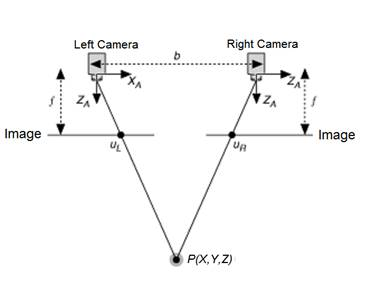
\includegraphics[height=60mm]{figures/stereoVisionDiagram.jpg}
		\captionfonts
		\caption{Simplified binocular stereo vision system~\cite{stereoVisionDiagram}.}
		\label{fig:sv_diagram}
	\end{center}
\end{figure}

The closer an object is to the stereo vision system, the greater the offset of corresponding pixels will be. If an object is too close to the system, it is possible for one camera to see part of an object that the other camera cannot. The farther an object is away from the stereo vision system, the smaller the offset of corresponding pixels. If an object is far enough away, it is possible for an object to be in almost the exact same location in both images. You can show this to yourself by holding a finger up close to your face, close one eye, and then alternate between which eye is open and which eye is closed. Your finger should appear to move a noticeable amount. Next, hold your finger as far away from you as you can and again alternate between which eye is open and which is closed. You should notice that your finger appears to move significantly less than it did when your finger was close to your face. That is how stereo vision works. The distance of an object is inversely proportional to the amount of offset between the two images.

\subsection{Parallelism in Stereo Vision}

Processing images for stereo vision allows for a high degree of parallelism. Locating the corresponding position of a pair of pixels is independent of finding another corresponding pair of pixels. This independence allows for the ability to process different parts of the same images at the same time, as long as there is hardware to support it.

Field Programmable Gateway Arrays (FPGAs) allow for a higher degree of parallel processing to be implemented compared to using the CPU on a computer. In Section~\ref{sec:impl} the amount of parallel processing used for the stereo vision module presented in this paper is discussed. 

\section{Stereo Vision Algorithms}

Stereo vision algorithms can be placed into one of 3 categories: pixel-based methods, area-based methods, and feature-based methods~\cite{xilinxSpartan3ABoard}. Pixel-based methods utilize pixel by pixel comparisons. They can produce dense disparity maps, but at the cost of higher computation complexity and higher noise sensitivity~\cite{xilinxSpartan3ABoard}. Area-based methods utilize block by block comparisons. They can produce dense disparity maps and are less sensitive to noise, however, accuracy tends to be low in areas that are not smooth~\cite{xilinxSpartan3ABoard}. Feature-based methods utilize features, such as edges and lines for comparisons. They cannot produce dense disparity maps, but have a lower computational complexity and are insensitive to noise~\cite{xilinxSpartan3ABoard}. 

There are a lot of different stereo vision algorithms~\cite{taxonomy}. In the taxonomy of~\cite{taxonomy}, 20 different stereo vision algorithms were compared against each other using various reference images. Many algorithms used are based on either the Sum of Absolute Differences (SAD) or correlation algorithms~\cite{alteraStratixIVPaper}.

An algorithm that is similar to SAD is the Sum of the Square Differences (SSD). Both of these algorithms produce similar results and contain around the same amount of error~\cite{xilinxSpartan3ABoard}. SAD was chosen over the other algorithms to implement in this paper because it is highly parallilizable and is simpler to implement in hardware. SSD requires squaring the difference between corresponding pixels and summing it up. Since squaring a number is the number multiplied by itself, the number will be added to itself that many times to produce the squared value. This causes more over head and more hardware is required than just taking the absolute value of the difference of a corresponding pair.

\subsection{Sum of the Absolute Differences (SAD) Algorithm}

SAD is a pixel-based matching method~\cite{alteraStratixIVPaper}. Stereo vision uses this algorithm to compare a group of pixels called a window from one image with a window in another image to determine if the corresponding center pixels match. The SAD algorithm, shown in Equation~\ref{eq:sadAlg1}~\cite{alteraStratixIVPaper}, takes the absolute difference between each pair of corresponding pixels and sums all of those values together to create a SAD value. One SAD value by itself does not give any useful information about the two corresponding center pixels. Several SAD values will be calculated from different candidate windows for each reference window. Out of the all the SAD values calculated for the reference window, the SAD value with the smallest value (all of them are greater than or equal to 0 because of the absolute part in the equation) is determined to contain the matching pixel. Figure~\ref{fig:sad_corr} shows that for one reference window, there are several candidate windows. The line that the candidate windows are chosen from called epipolar lines. 

\begin{equation}
	\sum\limits_{(i,j)\in W}\left| I_{1}(i,j)-I_{2}(x+i,y+j) \right|
	\label{eq:sadAlg1}
\end{equation}

\begin{figure}[h]
\begin{center}
	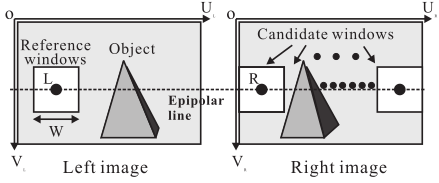
\includegraphics[height=50mm]{figures/sadCorrespondingWindows.png}
	\captionfonts
	\caption{Searching for corresponding points between the two images~\cite{sadParallel}.}
	\label{fig:sad_corr}
\end{center}
\end{figure}

In stereo vision, epipolar lines are created from the two cameras capturing images from the same scene. Figure~\ref{fig:epipolar} shows the epipolar line that point X must be on in the corresponding images. This is useful because if the epipolar lines are known for both images, then it is possible to know the line that two corresponding points are on. It reduces the problem of finding the same two points from a 2D area to a 1D line. Now, if the epipolar lines in both images are horizontal as they are in Fig.~\ref{fig:sad_corr} as opposed to them being at a diagonal as they are in Fig.~\ref{fig:epipolar}, then Eq.~\ref{eq:sadAlg1} reduces to Equation~\ref{eq:sadAlg2}. For cameras that are not perfectly aligned, rectification is often used in order to align epipolar lines between images~\cite{rectification}. However, many stereo vision algorithms will assume that the epipolar lines are rectified to simplify the overall processing required.

\begin{figure}[h]
\begin{center}
	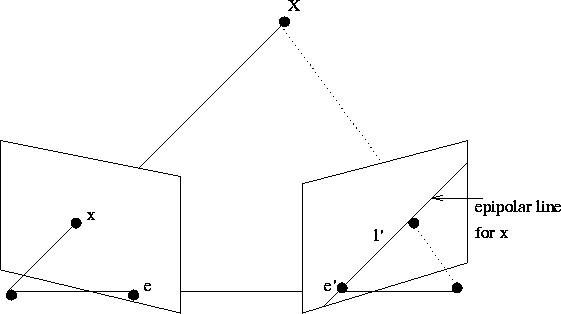
\includegraphics[height=55mm]{figures/epipolar.png}
	\captionfonts
	\caption{The epipolar line that point X is on for both images~\cite{epipolar}.}
	\label{fig:epipolar}
\end{center}
\end{figure}

\begin{equation}
	\sum\limits_{(i,j)\in W}\left| I_{1}(i,j)-I_{2}(x+i,j) \right|
	\label{eq:sadAlg2}
\end{equation}

The disparity is the amount of offset between two corresponding pixels. The disparity range is the number of pixels that the candidate window will move through the image and is represented by the value `x' in Eq.~\ref{eq:sadAlg2}. It corresponds to the amount of SAD values that will be calculated for each pixel. Figure~\ref{fig:sadGraphs} shows two types of SAD search methods. Fig.~\ref{fig:globalSAD} selects the overall SAD value with the lowest value to be the matching pixel. However, Fig.~\ref{fig:localSAD} limits the search region to a specific area. This helps to avoid issues of similar looking areas that are not near the reference window from being falsely identified as matching. The downside to this method is that if an object gets too close, meaning it would have high disparity values, and if the search region is not large enough, then the distance of the object will be miss classified. It is important to determine a window size and a search region that fit desired parameters.

For example, Figure~\ref{fig:template} shows a reference (template) window from one image.  Figure~\ref{fig:search} shows the candidate (search) area in from the other image. The disparity range is 3, or 0 to 2. There are three 3x3 windows within the search region in Fig.~\ref{fig:search}. From left to right the three search windows have their center pixel as 4, 6, and 5, respectively. 

\begin{figure}[h]
\begin{center}
	\begin{subfigure}{0.4\textwidth}
		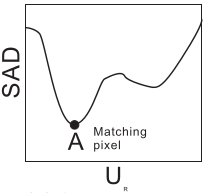
\includegraphics[width=\textwidth]{figures/sadGlobalGraph.png}
		\caption{Global SAD search}
		\label{fig:globalSAD}
	\end{subfigure}
	\begin{subfigure}{0.4\textwidth}
		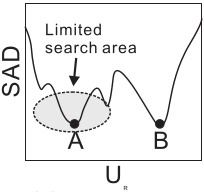
\includegraphics[width=\textwidth]{figures/sadLocalGraph.png}
		\caption{Local SAD search}
		\label{fig:localSAD}
	\end{subfigure}
	\captionfonts
	\caption{The SAD between a reference window and several candidate windows~\cite{sadParallel}.}
	\label{fig:sadGraphs}
\end{center}
\end{figure}

Comparing corresponding pixels in the template window with the first search window (S0) gives the absolute differences for all 9 pixels going from left to right and top to bottom of 8, 1, 1, 2, 1, 0, 1, 2, and 2. So the SAD value for S0 is 18, which is obtained by adding up all nine of those values. The SAD value for the second search window (S1) is 6 and the last search window (S2) is 13. The template window has the smallest SAD value with S1. Therefore the center pixel in S1 is determined to be the corresponding pixel for the center pixel in the template window. The disparity value is 1 (how far the matching search window was shifted to the right). The disparity value, along with many others, is used to create a disparity map. Each disparity value in the disparity map is at the same relative location that the center pixel of its corresponding template window is located.

\begin{figure}[h]
\begin{center}
	\begin{subfigure}{0.3\textwidth}
		\begin{center}				
			\begin{tabular}{|l|c|r|}
				\hline
				1 & 2 & 3 \\\hline
	  			4 & 5 & 6 \\\hline
		    	7 & 8 & 9 \\
		    	\hline
			\end{tabular}
		\end{center}
		\caption{Template Window}
		\label{fig:template}
	\end{subfigure}
	\begin{subfigure}{0.3\textwidth}
		\begin{center}		
			\begin{tabular}{|l|c|c|c|r|}
				\hline
				9 & 1 & 2 & 4 & 5 \\\hline
		  		2 & 4 & 6 & 5 & 3 \\\hline
		    	8 & 6 & 7 & 8 & 7 \\
		    	\hline
			\end{tabular}
		\end{center}
		\caption{Search Region}
		\label{fig:search}
	\end{subfigure}
	\captionfonts
	\caption{Template (reference) window and search (candidate) window.}
	\label{fig:windows}
\end{center}
\end{figure}
